%!TEX root = ../Electrodynamics.tex
\subsection{Волны в прямоугольном металлическом волноводе. Спектр собственных волновых чисел волн ТЕ и ТМ типов. Структура поля низших типов волн}


\paragraph{Решение для TM-волн.} Займемся решением TM-волны в прямоугольном волноводе (рис. \ref{fig:lect4:7}). Условимся что $a>b$. Эта задача поиска собственных функций $\phi^e$ и собственных значений $\varkappa$:
\begin{equation}
	\Delta_\perp \phi^e+\kappa^2\phi^e=0, \quad \phi^e|_l=0
\end{equation}

\begin{figure}[h!]
	\centering
	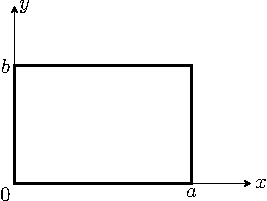
\includegraphics[scale=1.5]{img/lect4_ris7}
	\caption{Прямоугольный волновод}
	\label{fig:lect4:7}
\end{figure}

В матфизике эта задача о колебании мембраны с закрепленным краем. Она решается разделением переменных:
\begin{equation}
	\phi^e=X(x)\cdot Y(y)
\end{equation}
\begin{equation}
	\pdv[2]{\phi^e}{x}
		+\pdv[2]{\phi^e}{y}
			+\kappa^2 \phi^e =0  \quad \bigg| \cdot \frac{1}{XY}
	\quad \Rightarrow \quad
		\frac{X''}{X}+\frac{Y''}{Y}+\varkappa^2=0
\end{equation}

Тут надо произнести магическую фразу: так как первое слагаемое функция от $x$, второе функция от $y$, и их сумма равна константе для любых $x,y$, значит -- сами слагаемые тоже какие-то константы:
\begin{equation}
	\frac{X''}{X}=-\kappa_x^2, \quad
	\frac{Y''}{Y}=-\kappa_y^2
\end{equation}
Определив таким образом константы, мы получаем:
\begin{equation}
	\kappa_x^2+ \kappa_y^2=\kappa^2
\end{equation}
Пока мы не нашли само $\kappa$. Это собственное число, и оно подлежит определению. Прежде чем его найти, найдем собственные функции, решая уравнения
\begin{equation}
	X''+\kappa_x^2X=0, \quad Y''+\kappa_y^2Y=0
\end{equation}	
Это уравнения известного вида, их решение
\begin{equation}
	X=C_1\cdot\cos{\kappa_x x}+
		C_2\cdot\sin{\kappa_x x}
	\qquad
	Y=A_1\cdot\cos{\kappa_y y}+
		A_2\cdot\sin{\kappa_y y}	
\end{equation}
Нужно удовлетворить граничным условиям: 
\begin{equation}
	\phi^e|_{y=0}=0 \quad \Rightarrow \quad
		X(x)Y(0)=0 \quad \forall x \Rightarrow
		Y(0)=0 \quad \Rightarrow \quad A_1=0
\end{equation}
\begin{equation}
	\phi^e|_{x=0}=0 \quad \Rightarrow \quad
		X(0)Y(y)=0 \quad \forall y \Rightarrow
		X(0)=0 \quad \Rightarrow \quad C_1=0
\end{equation}
\begin{gather}
	\phi^e|_{x=a}=0 \quad \Rightarrow \quad
		X(a)Y(y)=0 \quad \forall y  \Rightarrow  \\ \Rightarrow
		X(a)=0 \quad \Rightarrow \quad \kappa_x a = m\pi, \quad m=\xcancel{0},1,2,\ldots
\end{gather}
Поскольку $m=0$ дает тривиальное решение, мы его откидываем.
\begin{gather}
	\phi^e|_{y=b}=0 \quad \Rightarrow \quad
		X(x)Y(b)=0 \quad \forall x  \Rightarrow  \\ \Rightarrow
		Y(b)=0 \quad \Rightarrow \quad \kappa_y b = n\pi , \quad n=\xcancel{0},1,2,\ldots
\end{gather}
Теперь мы получили выражения для $X$ и $Y$:
\begin{gather}
	X_m(x)=C_2\cdot\sin\frac{\pi m x}{a}\\
	Y_n(x)=A_2\cdot\sin\frac{\pi n y}{b}
\end{gather}
Теперь можем окончательно записать выражения для собственных функций и собственных значений в решении TM-волн:
\begin{gather}
	\label{phi_tm}
	\left.\begin{aligned}
		&\phi^e_{mn}=B_{mn}\sin\frac{\pi m x}{a}\sin\frac{\pi n y}{b}\\
		&\kappa_{mn}^2=\qty(\frac{m\pi}{a})^2+\qty(\frac{n\pi}{b})^2	
	\end{aligned}\right\}\,, \quad m,n=1,2,\ldots
\end{gather}
\paragraph{Решение для TE-волн.} Приведем решение без вывода:
\begin{gather}
	\label{phi_te}
	\left.\begin{aligned}
		&\phi^m_{mn}=B_{mn}\cos\frac{\pi m x}{a}\cos\frac{\pi n y}{b}\\
		&\kappa_{mn}^2=\qty(\frac{m\pi}{a})^2+\qty(\frac{n\pi}{b})^2	
	\end{aligned}\right\}\,, \quad m,n=(0),1,2,\ldots
\end{gather}
Важным отличием является то, что теперь одно из чисел $m,n$ может быть равно нулю (решение от этого не станет тривиальным).

\paragraph{Низшая мода.} По определению, низшая мода -- та, у которой минимальное поперечное волновое число. Так как мы предполагали, что $a>b$, то в нашем случае это мода TE$_{10}$:
\begin{equation}
	\kappa_{10}=\frac{\pi}{a} \quad \rightarrow \quad \omega_{cr\,10}=\frac{\kappa_{10}\cdot c}{\sqrt{\varepsilon \mu}} 	
\end{equation} 

Именно моду TE$_{10}$ чаще всего используют на практике в линиях передачи. 

Рассмотрим перпендикулярную структуру поля TE$_{10}$-волны. Нарисуем силовые линии полей $E$ и $H$ в плоскости $(x,y)$ -- перпендикулярной распространению волны (рис. \ref{fig:lect4:8})
\begin{figure}[h!]
	\centering
	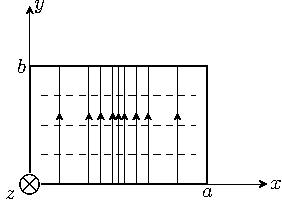
\includegraphics[scale=1.5]{img/lect4_ris8}
	\caption{Структура полей $\vec{E}$ и $\vec{H}$ ($\vec{H}$ изображено пунктиром)}
	\label{fig:lect4:8}
\end{figure}

На границах волновода поле $E$ равно нулю (в силу условия $E_\tau=0$). Поле $\vec{E}$ можем получить из уравнений \eqref{phi_te},\eqref{eperp}:
\begin{equation}
	\vec{E}=\vec{E}_\perp=\vec{y}_0E_0\cdot\sin\frac{\pi x}{a}\exp[i(\omega t - hz)],
\end{equation}
где 
\begin{equation}
	h=\sqrt{
		\frac{\omega^2}{c^2}\epsilon \mu - \qty(\frac{\pi}{a})^2
	}
\end{equation}

Поле $H$ можно найти из импедансного соотношения (для TE-волны):
\begin{equation}
	\frac{E_y}{H_x}=-\sqrt\frac{\mu}{\epsilon}\frac{k}{h}
\end{equation}

\begin{figure}[h!]
	\centering
	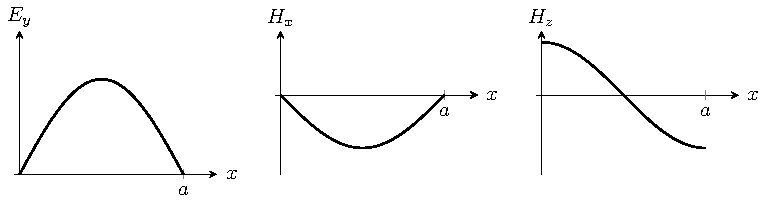
\includegraphics[width=\textwidth]{img/lect4_ris9}
	\caption{Поперечная структура полей $\vec{E}$ и $\vec{H}$ (мода TE$_{}$)}
	\label{fig:lect4:9}
\end{figure}

За перенос энергии отвечают именно поперечные компоненты поля. Компонента поля
$H_z \sim \cos\frac{\pi a}{x}$, а также сдвинута по фазе во времени. 

\begin{figure}[H]
	\centering
	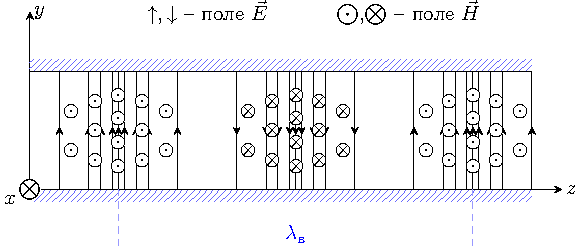
\includegraphics[width=\textwidth]{img/lect4_ris10}
	\caption{Продольная структура полей $\vec{E}$ и $\vec{H}$ (мода TE$_{}$)}
	\label{fig:lect4:10}
\end{figure}

\begin{figure}[H]
	\centering
	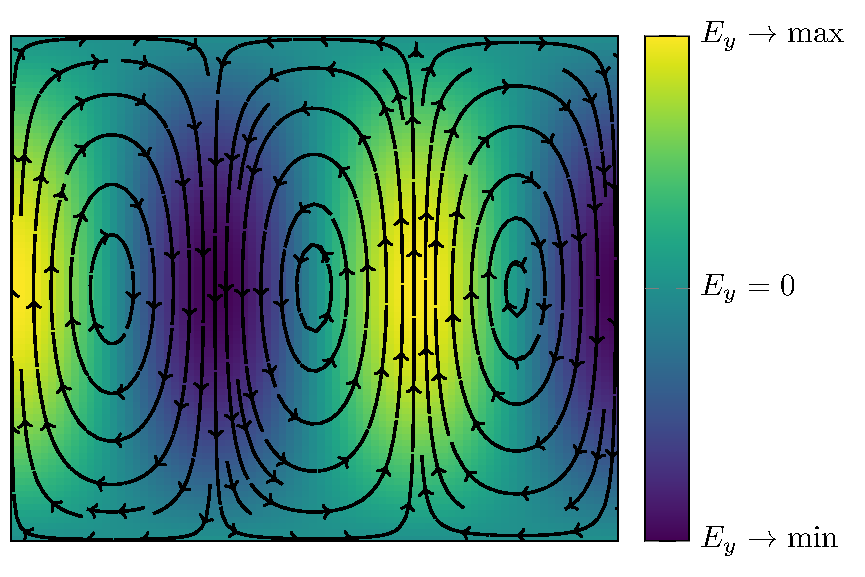
\includegraphics[scale=1]{img/lect4_ris11}
	\caption{Структура поля $\vec{H}$ (изображены силовые линии) и поля $\vec{E}$ (напряженность изображена цветом) волны TE$_{10}$ в прямоугольном волноводе}
	\label{fig:lect4:11}
\end{figure}

\paragraph{Высшие моды.} В зависимости от соотношения между $a$ и $b$, порядок мод может быть разным (он определяется величиной поперечного волнового числа). Некоторые высшие моды:
\begin{equation}
\begin{aligned}
 		\text{TE}_{11}:& \quad  \kappa_{11}=\sqrt{\qty(\frac{\pi}{a})^2+\qty(\frac{\pi}{b})^2}\\
 		\text{TE}_{20}:& \quad  \kappa_{20}=\frac{2\pi}{a} \\
 		\text{TE}_{01}:& \quad  \kappa_{11}=\frac{\pi}{b}
\end{aligned} 	
\end{equation} 


\subsection{Затухание собственных колебаний в полом резонаторе, обусловленное потерями энергии в заполняющей среде}